\documentclass[12pt]{article}
\usepackage{amsmath}
\usepackage{amssymb}
\usepackage{geometry}
\usepackage{enumerate}
\usepackage{natbib}
\usepackage{float}%稳定图片位置
\usepackage{graphicx}%画图
\usepackage[english]{babel}
\usepackage{a4wide}
\usepackage{indentfirst}%缩进
\usepackage{enumerate}%加序号
\usepackage{multirow}%合并行
\title{\large UM-SJTU JOINT INSTITUTE\\Advanced Lasers and Optics Laboratory\\(VE438)\\\ \\\ \\\ \\\ \\\ \\\ \\\ \\\ \\\ \\\ \\\
Pre Lab Assignment\\\ \\\ LAB 7\\\ Liquid Crystal Display \\\ \\\ \\\ \\\ \\\ }
\author{Name: Pan Chongdan \\ID: 516370910121}
\date{Date: \today}

\begin{document}
\maketitle
\newpage
\section{Answers for Pre Lab Questions}
\subsection{Question 1}
\begin{figure}[H]
\centering
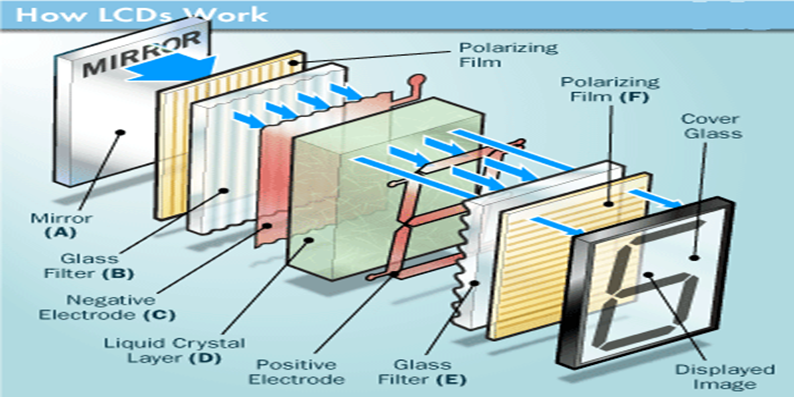
\includegraphics[scale=0.5]{P1.png}
\end{figure}
For LCD displayer, the liquid crystal layer is put between the negative electrode and positive electrode. When the electric field is formed between the two electrodes, the liquid crystal molecular will be distorted so that we can control the reflection and brightness of the light because the light's polarization direction has been changed by the molecular. The glass filter can be used to produce different colors of the light. The LCD can't emit the light by it self, but it can control the light passing through by control its polarization.
\subsection{Question 2}
When there is no voltage, the light will be polarized by the liquid crystal molecular for 90 degree and it can pass through the two perpendicularly polarized layers. When there is voltage applied, the liquid crystal molecular will be aligned in one direction parallel to the light's direction so that it can't change the polarization direction of the light. As a result, the light can't pass the second polarized layers because their polarization directions are perpendicular to each other. In conclusion, when there is voltage, the light won't be polarized and can't pass through the layer and vice versa.
\end{document}